\section*{Appendix D: Tool Usage}
\label{appendixD}

In this section we demonstrate how to use TMACS to show that the specification and 
implementation of the alternating bit protocol, as described in Section~\ref{sec:application} are weakly bisimiliar. 
As a first step we always need to generate the labeled transition systems for both the specification and the 
implementation of the system that we are trying to model. That can be done in the tab "CCS to LTS" in the tool. 
As shown in Fig.~\ref{fig:abptoolusage1} in the upper text area we need to write down the CCS 
expressions that describe the system or load them from a file. One constraint here
is that a general CCS expression that describes the whole system has to be put on
the first line. The algorithm for generating the labeled graph performs the evaluation and the 
construction of the graph starting from the first line. When we have our CCS expressions
put in place we have to click "Generate LTS". This action will make the application
parse the expression and if no errors are found it will start generating the labeled graph.
The results from the generated graph will be presented in Aldebaran format in the lower text area. 
The users can save the results in a file or can click "View LTS Graph" 
which causes the tool to display a computer generated image of the labeled graph.

\begin{figure}[!ht]
\centering
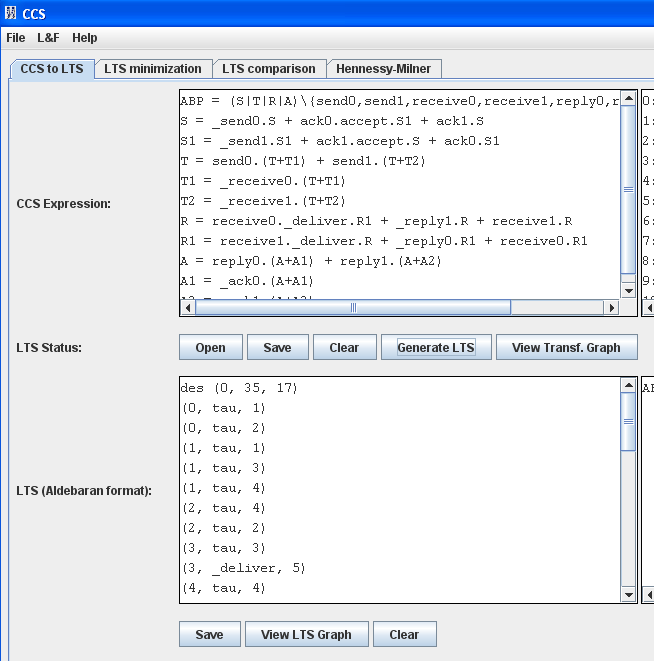
\includegraphics[width=5in]{ABPToolUsage1}
\caption{TMACS usage: ABP modeling and generating the respective labeled transition system in Aldebaran format}
\label{fig:abptoolusage1}
\end{figure}

Reduction of the state space of a labeled transition system can be done in the "LTS minimization" tab. The minimization is pretty 
straigthforward process. As shown in Fig.~\ref{fig:abptoolusage2} and Fig.~\ref{fig:abptoolusage3}
the labeled transtion system is loaded from an Aldebaran file, a method of calculation is chosen and the user has to click the button "Calculate" in order to perform calculation.

\begin{figure}[!ht]
\centering
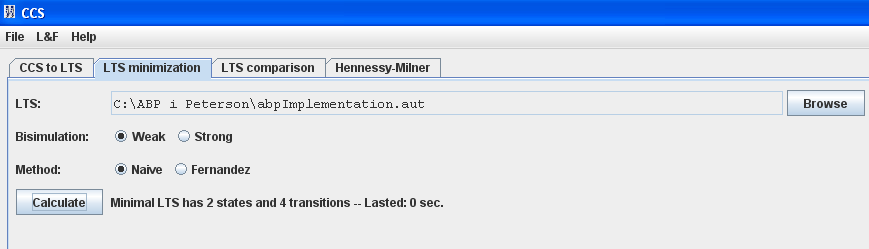
\includegraphics[width=5in]{ABPToolUsage2}
\caption{TMACS usage: ABP minimization, using weak bisimilarity and the naive algorithm for computing strong bisimulation equivalence}
\label{fig:abptoolusage2}
\end{figure}

\begin{figure}[h]
\centering
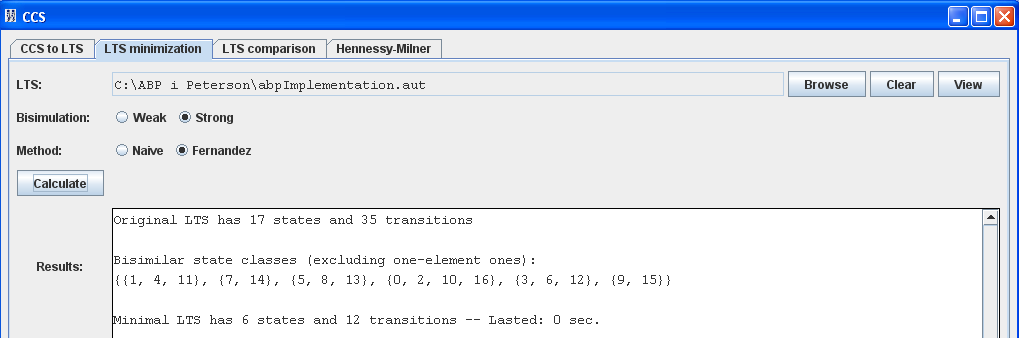
\includegraphics[width=5in]{ABPToolUsage3}
\caption{TMACS usage: ABP minimization, using strong bisimilarity and the algorithm of Fernandez for computing strong bisimulation equivalence}
\label{fig:abptoolusage3}
\end{figure}

Checking for labeled transition system bisimilarity is performed in the "LTS comparison" tab. This tab is 
similar to the one for the minimization. As shown in Fig.~\ref{fig:abptoolusage4} and
Fig.~\ref{fig:abptoolusage5} two labeled transition systems have to be loaded from Aldebaran files. In order to perform comparison of the two labeled transition systems with respect to strong or weak bisimulation equivalence, the user has to choose a method for calculation and then click the button 
"Calculate". The results will be displayed on the right side of the button and they
give information whether the labeled transition systems are strongly/weakly bisimilar and how long the calculation lasted.

\begin{figure}[!ht]
\centering
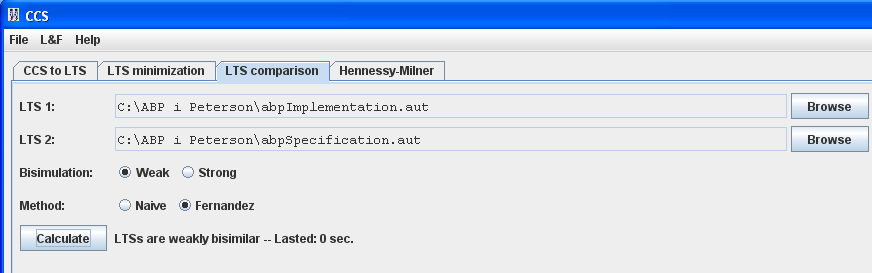
\includegraphics[width=5in]{ABPToolUsage4}
\caption{TMACS usage: ABP comparison, using weak bisimilarity and the algorithm of Fernandez for computing strong bisimulation equivalence}
\label{fig:abptoolusage4}
\end{figure}

\begin{figure}[!ht]
\centering
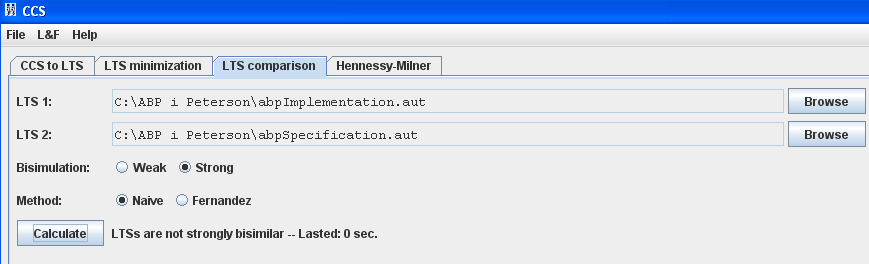
\includegraphics[width=5in]{ABPToolUsage5}
\caption{TMACS usage: ABP comparison, using strong bisimilarity and the naive algorithm for computing strong bisimulation equivalence}
\label{fig:abptoolusage5}
\end{figure}

TMACS also gives possibility to check whether certain Hennessy-Milner logic expression is valid for a given labeled transition system in Aldebaran format. That is done via the "Hennessy-Milner" tab. The labeled transition system is loaded from an Aldebaran file and then the user needs to enter Hennessy-Milner logic recursive formula which uses $U^{w}$ and/or $U^{s}$ operator. By clicking on the "Calculate" button, a true/false answer is given meaning that the Hennessy-Milner expression is valid or not for the input labeled transition system. This process is shown on Fig.~\ref{fig:hml1} and Fig.~\ref{fig:hml2}.

\begin{figure}[!ht]
\centering
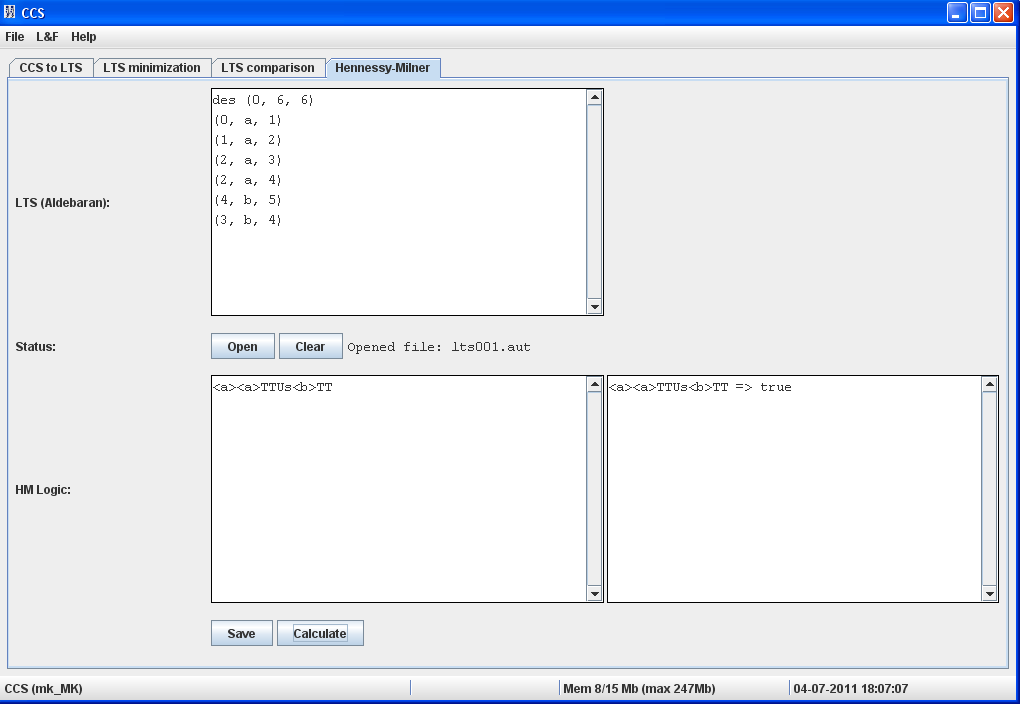
\includegraphics[width=5in]{hml1}
\caption{TMACS usage: checking validity of a recursive Hennessy-Milner logic formula for an input labeled transition system}
\label{fig:hml1}
\end{figure}

\begin{figure}[!ht]
\centering
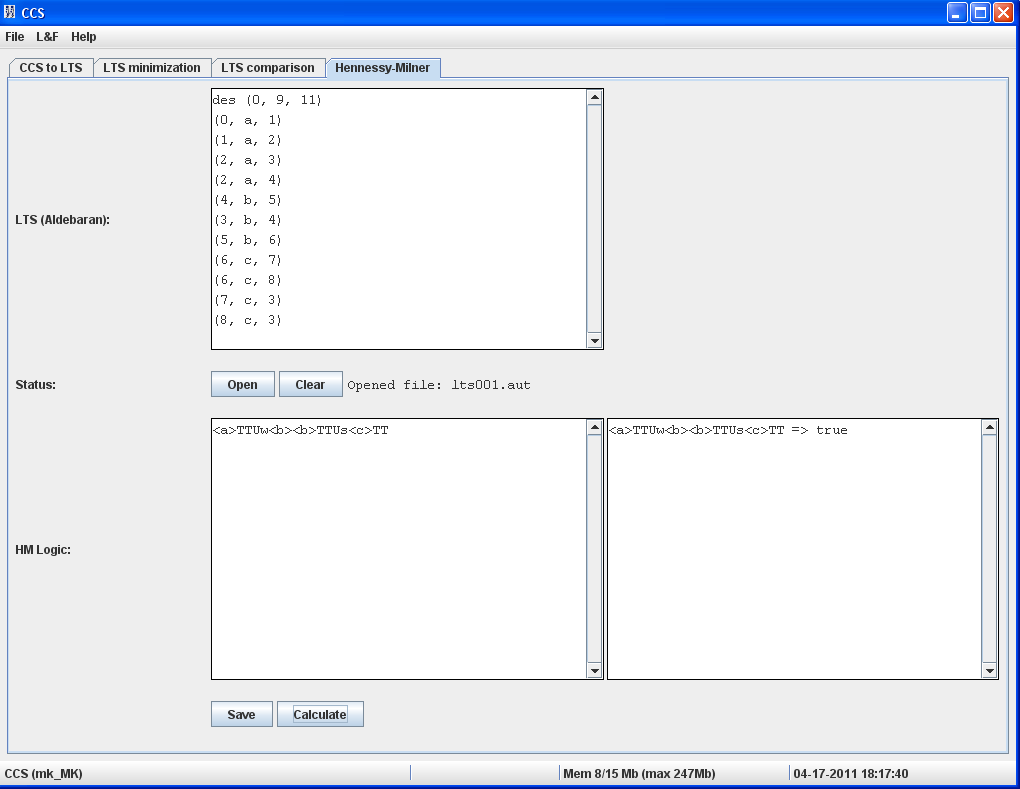
\includegraphics[width=5in]{hml2}
\caption{TMACS usage: checking validity of a recursive Hennessy-Milner logic formula for an input labeled transition system}
\label{fig:hml2}
\end{figure}